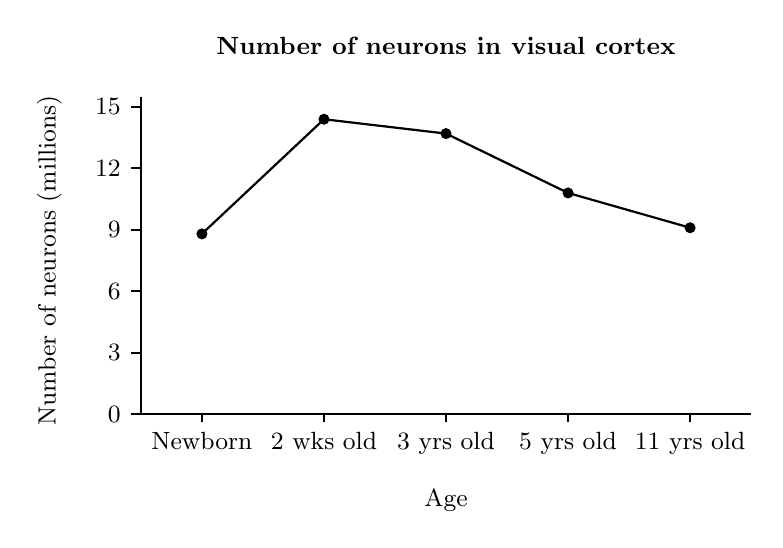
\begin{tikzpicture}[x=1.55cm,y=0.26cm,font=\small]
\node[font=\small\bfseries] at (2,18) {Number of neurons in visual cortex};
% axes
\draw[thick] (-0.5,0) -- (4.5,0);
\draw[thick] (-0.5,0) -- (-0.5,15.5);
\foreach \y in {0,3,6,9,12,15} {\draw[thick] (-0.5,\y) -- (-0.58,\y) node[left] {\y};}
\foreach \x/\l in {0/Newborn,1/2 wks old,2/3 yrs old,3/5 yrs old,4/11 yrs old} {
  \draw[thick] (\x,0) -- (\x,-0.4) node[below] {\l};
}
\node at (2,-4.2) {Age};
\node[rotate=90] at (-1.25,7.5) {Number of neurons (millions)};
% data
\draw[thick] (0,8.8) -- (1,14.4) -- (2,13.7) -- (3,10.8) -- (4,9.1);
\foreach \x/\y in {0/8.8,1/14.4,2/13.7,3/10.8,4/9.1} {\fill (\x,\y) circle (2pt);}
\end{tikzpicture}
